\documentclass[11pt,a4paper]{article}
\usepackage[utf8]{inputenc}
\usepackage{amsmath}
\usepackage{graphicx}
\usepackage{listings}
\usepackage{xcolor}

% Code snippet styling
\definecolor{codegreen}{rgb}{0,0.6,0}
\definecolor{codegray}{rgb}{0.5,0.5,0.5}
\definecolor{codepurple}{rgb}{0.58,0,0.82}
\definecolor{backcolour}{rgb}{0.95,0.95,0.92}

\lstset{
    backgroundcolor=\color{backcolour},   
    commentstyle=\color{codegreen},
    keywordstyle=\color{magenta},
    numberstyle=\tiny\color{codegray},
    stringstyle=\color{codepurple},
    basicstyle=\ttfamily\footnotesize,
    breakatwhitespace=false,         
    breaklines=true,                 
    captionpos=b,                    
    keepspaces=true,                 
    numbers=left,                    
    numbersep=5pt,                  
    showspaces=false,                
    showstringspaces=false,
    showtabs=false,                  
    tabsize=2
}

\title{Short Report: Total Pressure Field Implementation in OpenFOAM}
\author{Fluid Dynamics Assignment}
\date{\today}

\begin{document}

\maketitle

\section{Introduction}
The objective of this task is to compute the total pressure field $p_{\text{total}}$ within the \texttt{pitzDaily} tutorial case using a runtime \texttt{codedFunctionObject}. The total pressure is defined mathematically as:
\begin{equation}
    p_{\text{total}} = p + \frac{1}{2}|\mathbf{U}|^2
\end{equation}
Where $p$ represents the static pressure field, and $\frac{1}{2}|\mathbf{U}|^2$ represents the dynamic pressure component (normalized by density $\rho$ for incompressible flow simulation).

\section{Implementation in \texttt{controlDict}}
To avoid modifying the core solver source code, a dynamic C++ function object was written inside the \texttt{system/controlDict} file. The snippet reads both fields from the database, executes the algebraic expression on every cell volume, and writes out the resulting field at every designated output interval.

\begin{lstlisting}[language=C++, caption=Coded function object code inside controlDict]
p_total
{
    type            coded;
    libs            (utilityFunctionObjects);
    name            p_total;
    writeControl    writeTime;

    codeWrite
    #{
        const volScalarField& p = mesh().lookupObject<volScalarField>("p");
        const volVectorField& U = mesh().lookupObject<volVectorField>("U");

        volScalarField p_total
        (
            IOobject
            (
                "p_total",
                mesh().time().timeName(),
                mesh(),
                IOobject::NO_READ,
                IOobject::AUTO_WRITE
            ),
            p + 0.5 * magSqr(U)
        );

        p_total.write();
    #};
}
\end{lstlisting}

\section{Results and Plotting}
After running the case using \texttt{pimpleFoam}, the newly written field files \texttt{p\_total} were verified in the time directories. The output results can be viewed visually in ParaView or extracted along a specific pathline to generate custom spatial plots.

Uncomment and include your plot below when ready:
\begin{figure}[htbp]
    \centering
    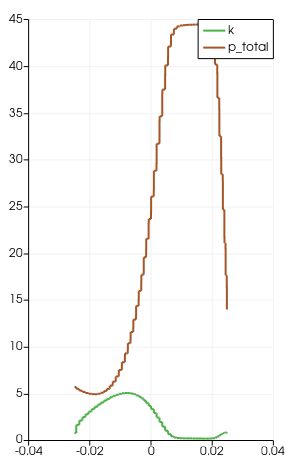
\includegraphics[width=0.8\textwidth]{p_total_line-plot.png}
   \caption{Total Pressure profile distribution at Time 0.3 sec across the pitzDaily channel geometry.}
   \label{fig:p_total}
\end{figure}
\begin{figure}[htbp]
    \centering
    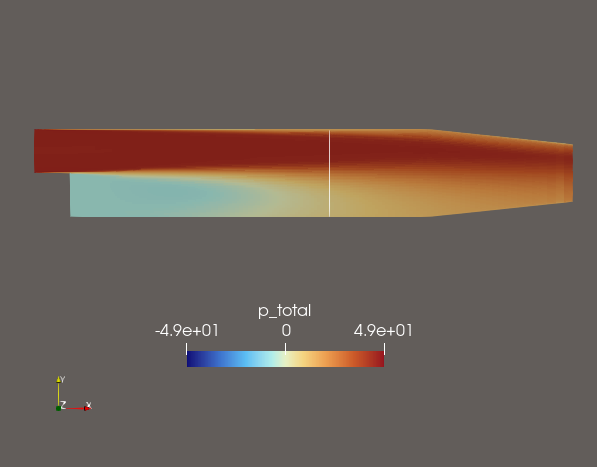
\includegraphics[width=0.8\textwidth]{p_total.png}
   \caption{Total Pressure at Time 0.3 sec in the pitzDaily channel geometry.}
   \label{fig:p_total}
\end{figure}
\begin{figure}[htbp]
    \centering
    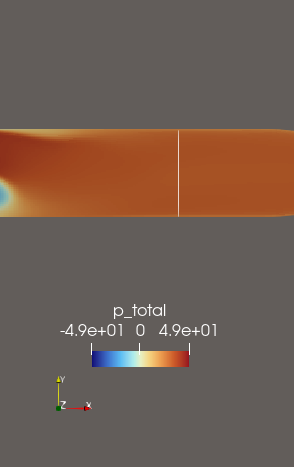
\includegraphics[width=0.8\textwidth]{p_total_line-plot 0.02.png}
   \caption{Total Pressure profile distribution at Time 0.02 sec across the pitzDaily channel geometry.}
   \label{fig:p_total}
\end{figure}
\begin{figure}[htbp]
    \centering
    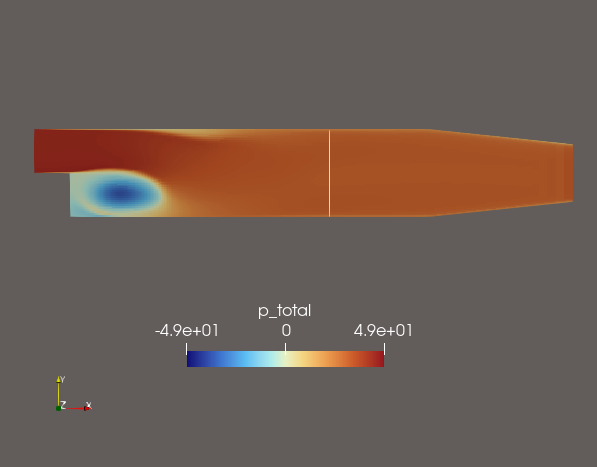
\includegraphics[width=0.8\textwidth]{p_total 0.02.png}
   \caption{Total Pressure at Time 0.02 sec in the pitzDaily channel geometry.}
   \label{fig:p_total}
\end{figure}
\begin{figure}[htbp]
    \centering
    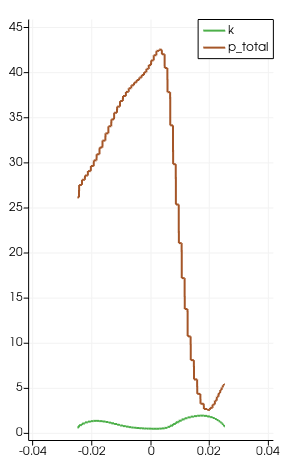
\includegraphics[width=0.8\textwidth]{p_total_line-plot 0.05.png}
   \caption{Total Pressure profile distribution at Time 0.05 sec across the pitzDaily channel geometry.}
   \label{fig:p_total}
\end{figure}
\begin{figure}[htbp]
    \centering
    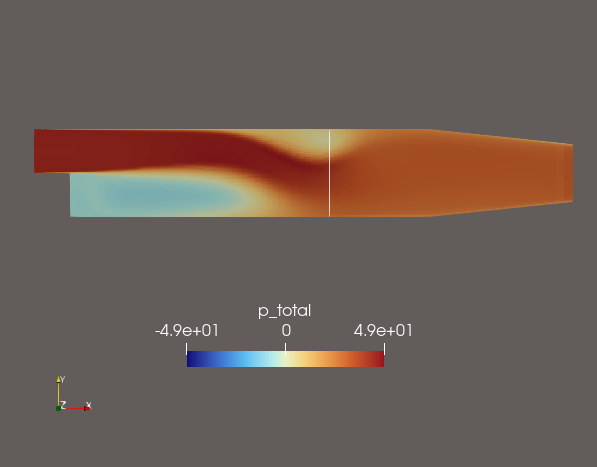
\includegraphics[width=0.8\textwidth]{p_total 0.05.png}
   \caption{Total Pressure at Time 0.05 sec in the pitzDaily channel geometry.}
   \label{fig:p_total}
\end{figure}
\begin{figure}[htbp]
    \centering
    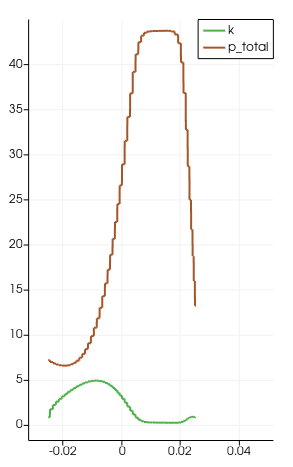
\includegraphics[width=0.8\textwidth]{p_total_line-plot 0.1.png}
   \caption{Total Pressure profile distribution at Time 0.1 sec across the pitzDaily channel geometry.}
   \label{fig:p_total}
\end{figure}
\begin{figure}[htbp]
    \centering
    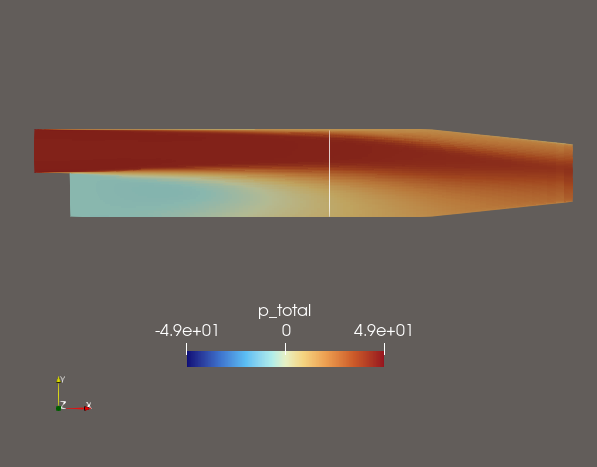
\includegraphics[width=0.8\textwidth]{p_total 0.1.png}
   \caption{Total Pressure at Time 0.1 sec in the pitzDaily channel geometry.}
   \label{fig:p_total}
\end{figure}

\end{document}
